\chapter[Dataset]{Dataset}
\markboth{Chap. 3\ \ \enspace Experimental methods}{Chap 2. Experimental methods}

\regularsection
\headerregularsection

\updatemylof % to be used with "list of figure divider per chapter" (see PREAMBLE)
\updatemylot % to be used with "list of table divider per chapter" (see PREAMBLE)

\begin{sloppypar} % to suppress overfull box

  Our new benchmark has 100000 cropped images after discarding some of the images only containing background. Of these, 10000 contain 30000 traffic signs in total. Although our source images cover much of Bangladesh and India, an imbalance still exists between different classes of traffic sign in our benchmark. This is unavoidable: classes such as signs. It can be from different viewpoints, have different ground sampling distances (gsd), different image sizes, aspect ratios, color, etc. Vehicles in different data may be significantly different in size and appearance. Figure~\ref{fig:figures/paper/dataset/collage.jpg} shows different images from four different datasets. It is obvious how different the VOC data is from any of the elevated data, while the VEDAI and AFVID data are somewhat similar, and the AF Build-ing Camera data is more similar to the aerial and satellite data. A more detailed look at the aerial datasets is available in TableNumber of classesIn the configuration file that defines the YOLO net model there is a 'classes' definition that is used to define the number of classes. To change the number of classes used, more than just the classes setting will need to be changed; the number of filters in the last convolutional layer must be altered to reflect the changed number of classes. The number of filters is set by $num(classes + coords + 1)$, where num isnumber of anchor boxes, and coords is four corresponding to the four coordinates used to define a bounding box.

\end{sloppypar}

\begin{figure}[H] % \begin{figure}[H] for forcing the figure placement here ; in the bottom, \begin{figure}[!b] ; top of the page, \begin{figure}[!t] ; otherwise, \begin{figure} will let LaTeX decide the best figure placement for you
  \centering
  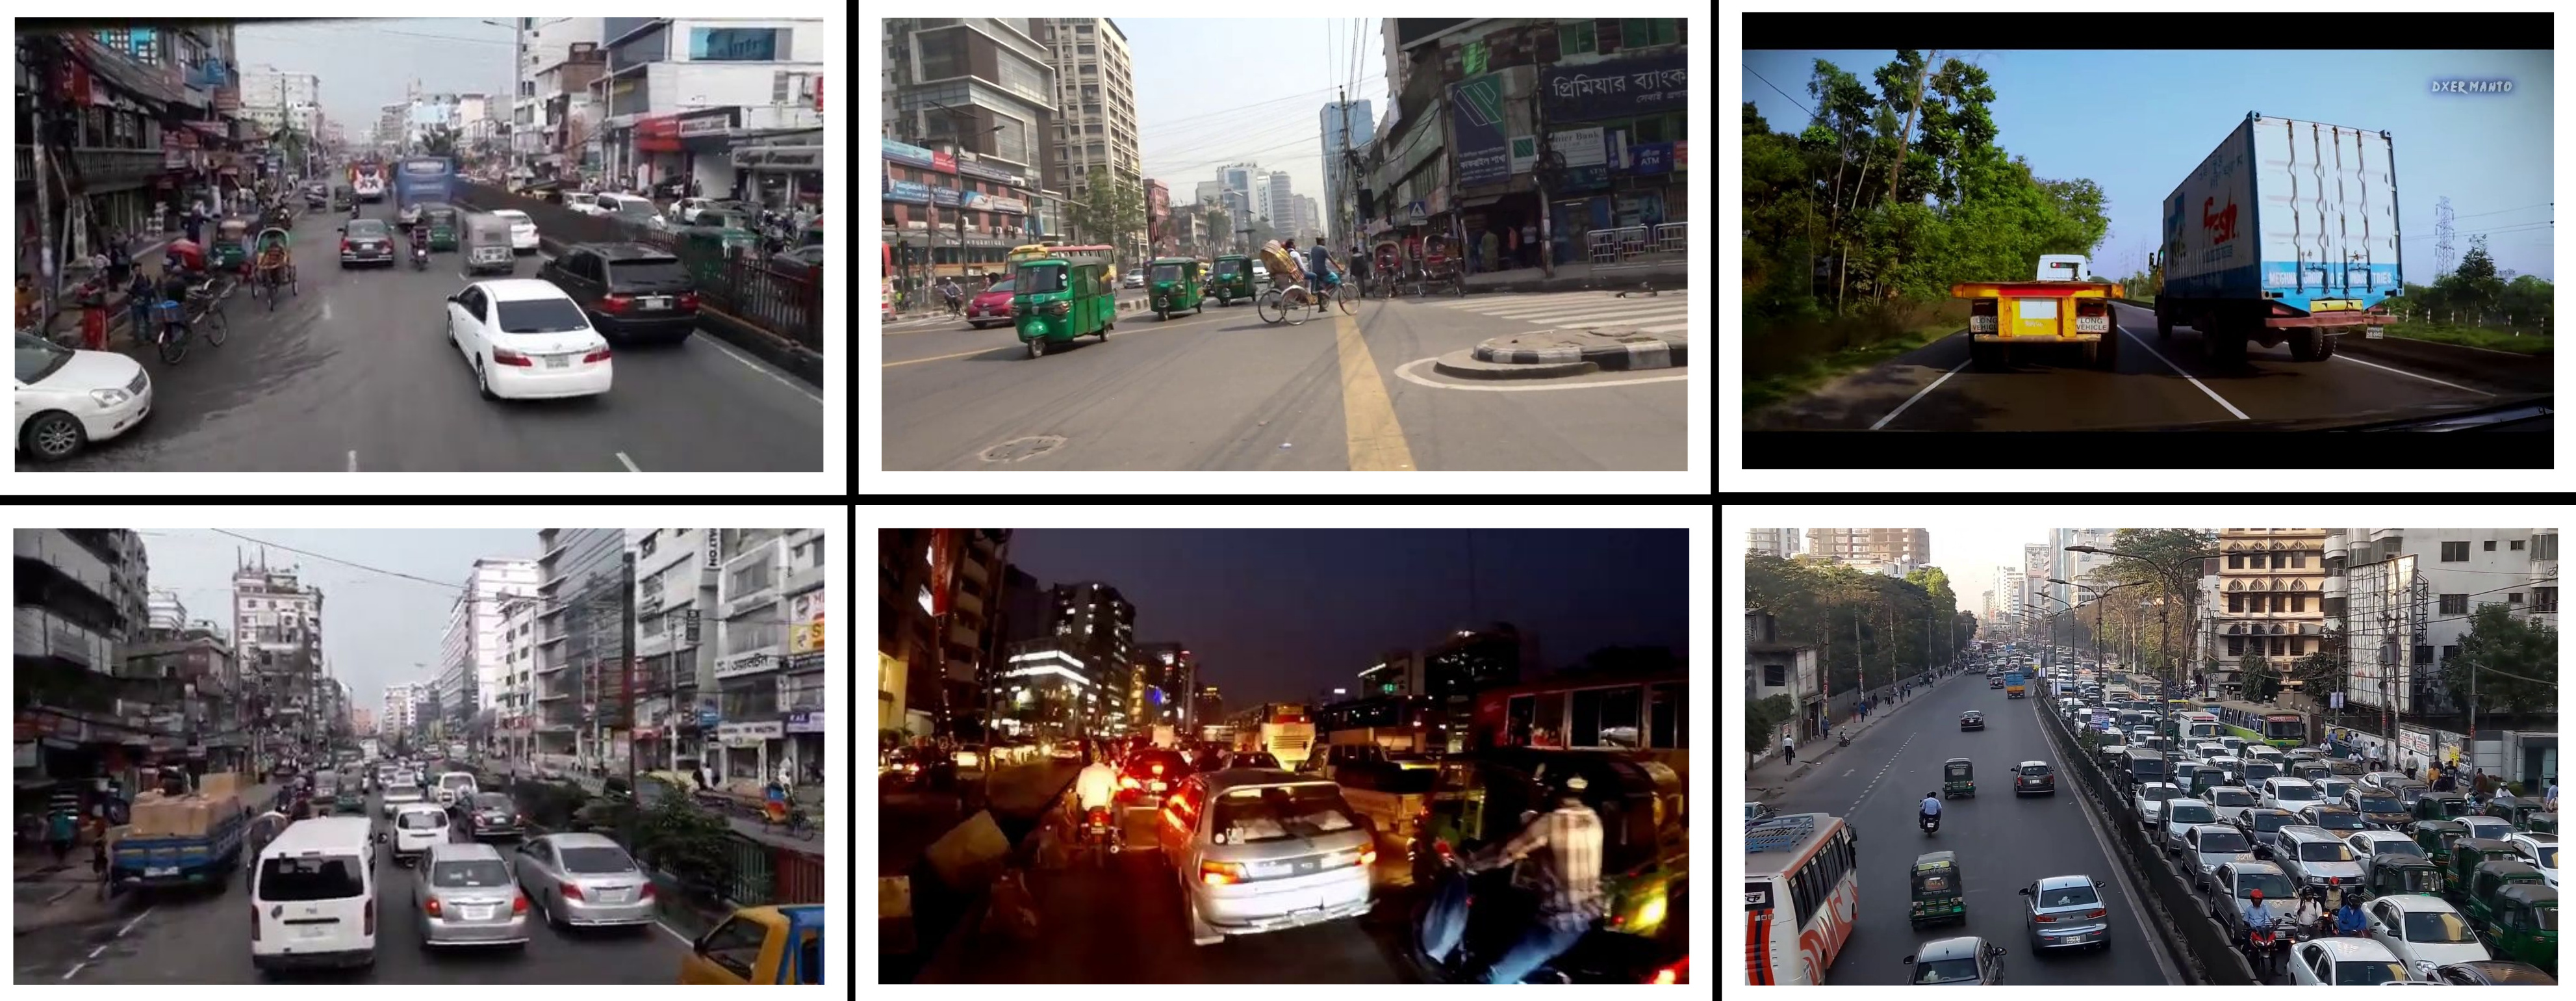
\includegraphics[width=\textwidth]{figures/paper/dataset-collage.jpg}
  \caption[Dataset Collage]{\textbf{Dataset Collage}. Some sample data from Dhaka AI dataset.}
  \label{fig:figures/paper/dataset-collage.jpg}
\end{figure}



\section{COCO Dataset Details}
\begin{itemize}
  \item \textbf{Images per class} ≥ 1500 images per class recommended
  \item \textbf{Instances per class} ≥ 10000 instances (labeled objects) per class recommended
  \item \textbf{Image variety} Must be representative of deployed environment. For real-world use cases we recommend images from different times of day, different seasons, different weather, different lighting, different angles, different sources (scraped online, collected locally, different cameras) etc.
 \item \textbf{Label consistency} All instances of all classes in all images must be labelled. Partial labelling will not work.
 \item \textbf{Label accuracy} Labels must closely enclose each object. No space should exist between an object and it's bounding box. No objects should be missing a label.
 \item \textbf{Background images} Background images are images with no objects that are added to a dataset to reduce False Positives (FP). We recommend about 0-10\% background images to help reduce FPs (COCO has 1000 background images for reference, 1\% of the total). No labels are required for background images.
\end{itemize}


\section{Dhaka AI Dataset}
We have used  a mixed dataset from Indian Driving Dataset and Dhaka AI Traffic Detection Challenge Dataset. 
\begin{figure}[H] % \begin{figure}[H] for forcing the figure placement here ; in the bottom, \begin{figure}[!b] ; top of the page, \begin{figure}[!t] ; otherwise, \begin{figure} will let LaTeX decide the best figure placement for you
  \centering
  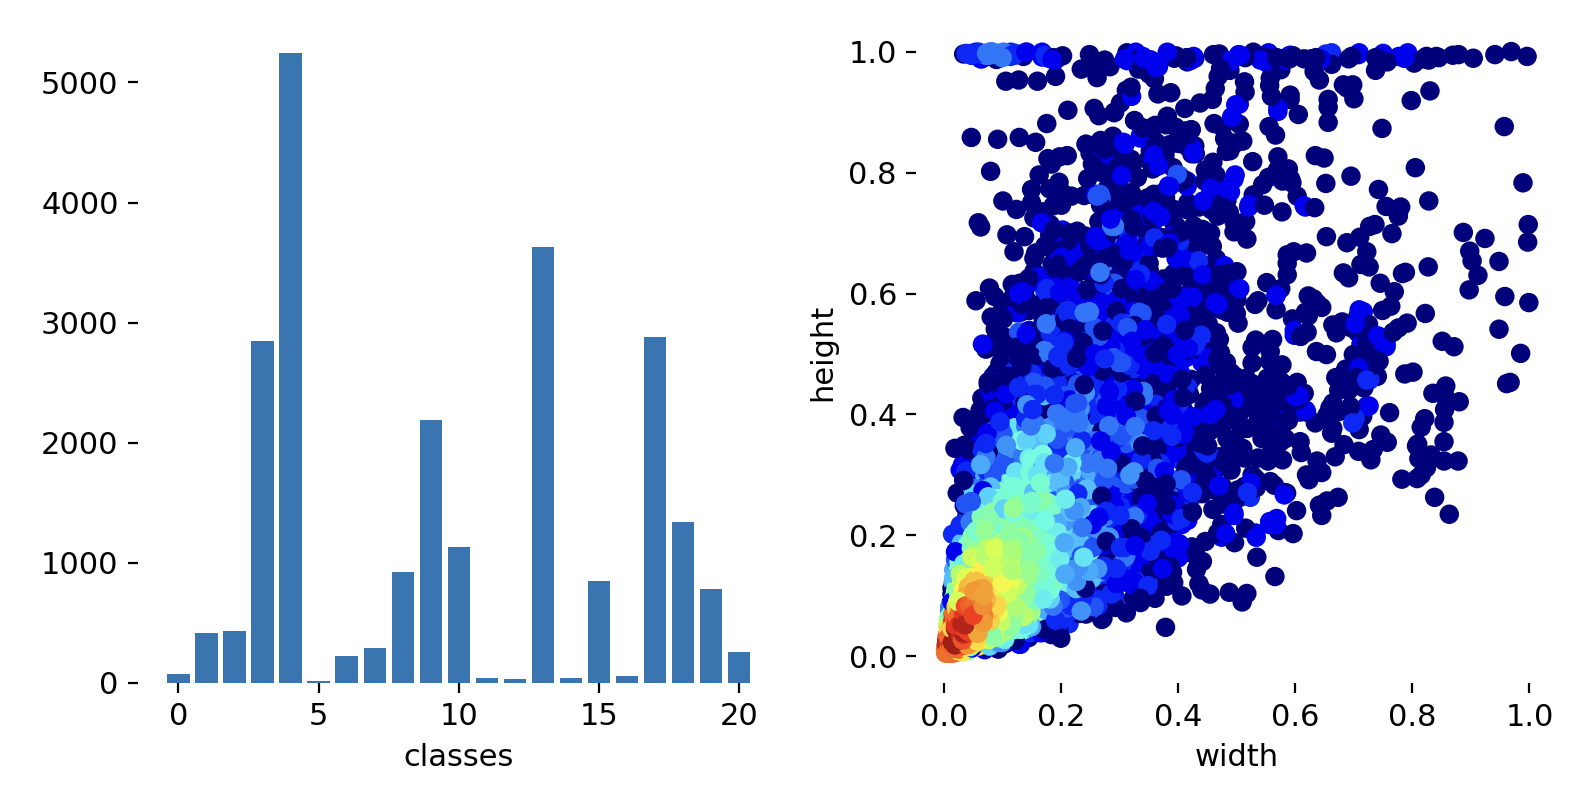
\includegraphics[width=\textwidth]{figures/paper/dhaka-ai+idd.png}
  \caption[Dataset Collage]{\textbf{Dataset Collage}. Some sample data from Dhaka AI dataset.}
  \label{fig:figures/paper/dhaka-ai+idd.png}
\end{figure}


\begin{figure}[H] % \begin{figure}[H] for forcing the figure placement here ; in the bottom, \begin{figure}[!b] ; top of the page, \begin{figure}[!t] ; otherwise, \begin{figure} will let LaTeX decide the best figure placement for you
  \centering
  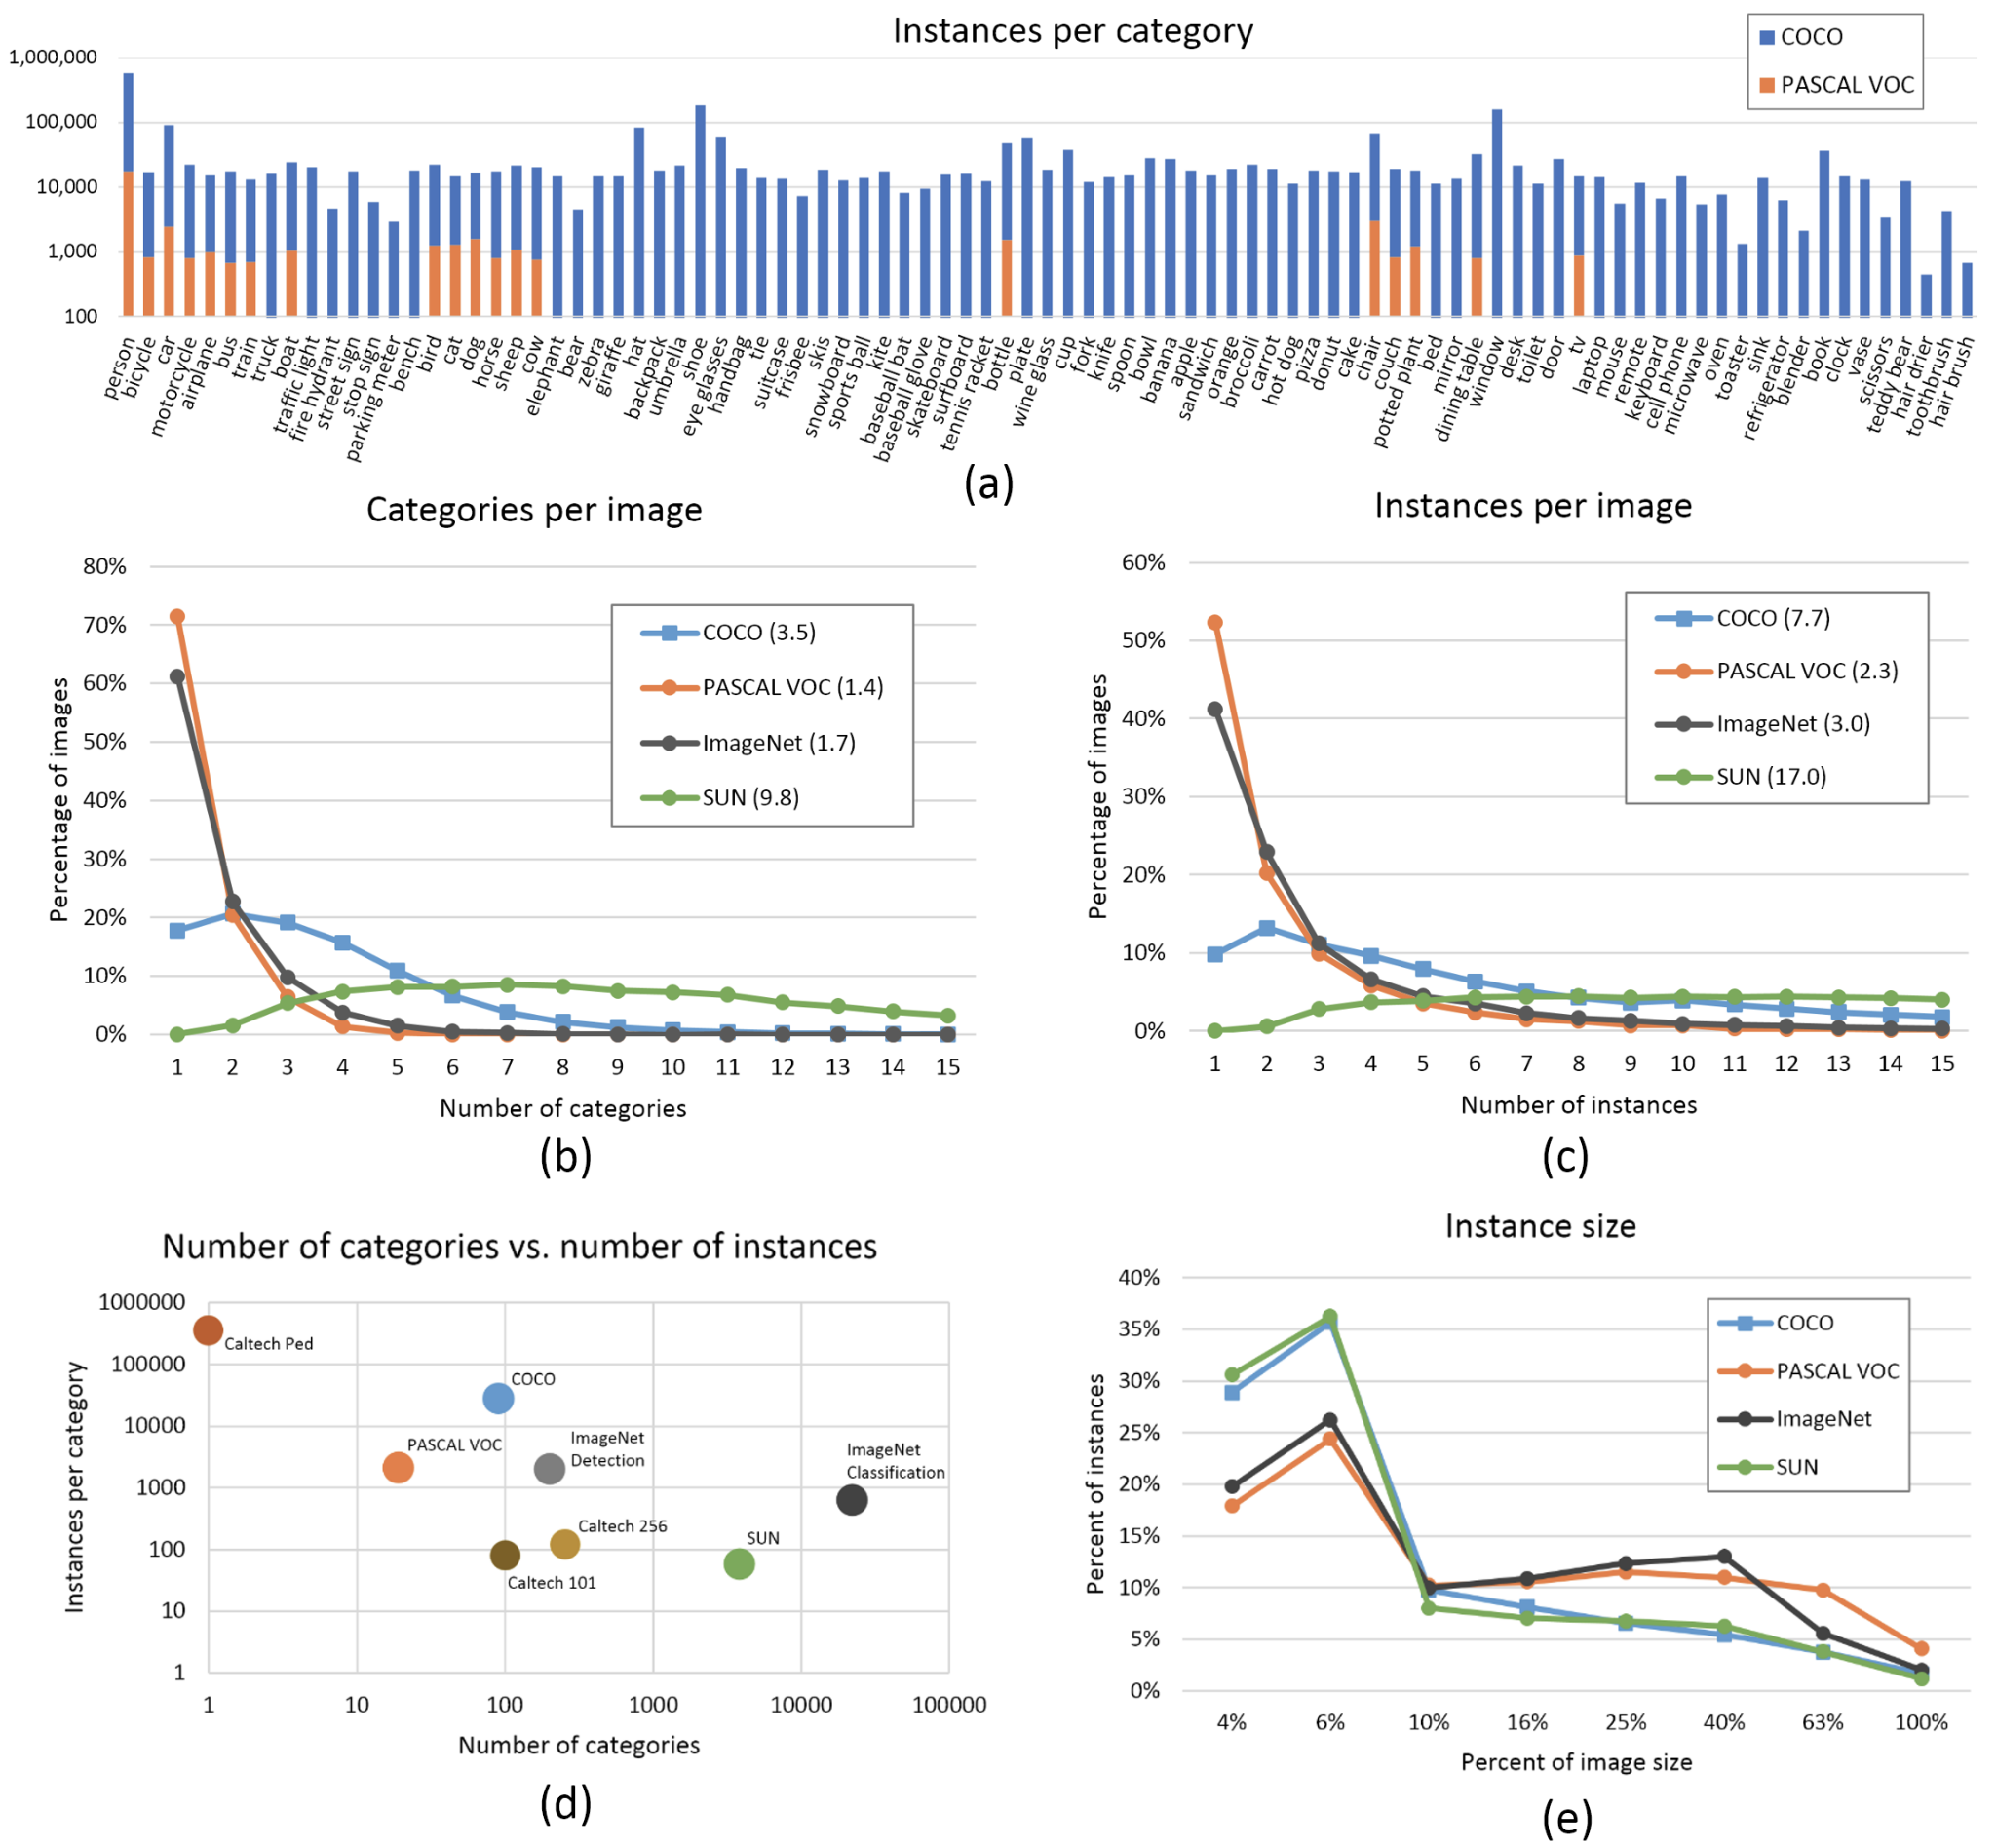
\includegraphics[width=\textwidth]{figures/paper/coco-details.png}
  \caption[Dataset Collage]{\textbf{Dataset Collage}. Some sample data from Dhaka AI dataset.}
  \label{fig:figures/paper/coco-details.png}
\end{figure}



\subsection{List of classes}
\begin{multicols}{2}
\begin{itemize}
\item Ambulance
\item Auto Rickshaw
\item Bicycle
\item Bus
\item Car
\item Garbage Van
\item Human Hauler
\item Minibus
\item Minivan
\item Motorbike
\item Pickup
\item Army Vehicle
\item Police Car
\item Rickshaw
\item Scooter
\item SUV
\item Taxi
\item Three Wheelers (CNG)
\item Truck
\item Van
\item Wheelbarrow
\end{itemize}
\end{multicols}


\section{Training Settings}
Before modifying anything, first train with default settings to establish a performance baseline. A full list of train.py settings can be found in the train.py argparser.
\begin{itemize}
  \item \textbf{Epochs} Start with 300 epochs. If this overfits early then you can reduce epochs. If overfitting does not occur after 300 epochs, train longer, i.e. 600, 1200 etc epochs.
  \item \textbf{Image size} COCO trains at native resolution of \texttt{--img 640}, though due to the high amount of small objects in the dataset it can benefit from training at higher resolutions such as \texttt{--img 1280}. If there are many small objects then custom datasets will benefit from training at native or higher resolution. Best inference results are obtained at the same \texttt{--img} as the training was run at, i.e. if you train at \texttt{--img 1280} you should also test and detect at \texttt{--img 1280}.
  \item \textbf{Batch size} Use the largest \texttt{--batch-size} that your hardware allows for. Small batch sizes produce poor batchnorm statistics and should be avoided.
  \item \textbf{Hyperparameters} Default hyperparameters are in \texttt{hyp.scratch.yaml}. We recommend you train with default hyperparameters first before thinking of modifying any. In general, increasing augmentation hyperparameters will reduce and delay overfitting, allowing for longer trainings and higher final mAP. Reduction in loss component gain hyperparameters like \texttt{hyp['obj']} will help reduce overfitting in those specific loss components.
\end{itemize}


%=======================================================================
%%% References

% \clearpage
\phantomsection
\specialsection % put an indent, see preamble
\headerspecialsection

{\hypersetup{urlcolor=ntnu,linkcolor=sophia} % set clickable URL title color to black, not ntnu like in the main document

  \bibliographystyle{unsrtnat-mod}  % NATBIB ref style
  \bibliography{references}
}
